\documentclass[a4paper,10pt]{article}

% Encoding and typeface: XeLaTeX with Latin Modern Roman (fontspec default), Turkish via polyglossia
\usepackage{fontspec}
\usepackage{polyglossia}
\setdefaultlanguage{turkish}

% Layout (tight margins)
\usepackage[a4paper,top=1.2cm,bottom=1.3cm,left=1.3cm,right=1.3cm]{geometry}

% Typography
\usepackage{microtype}
\usepackage{setspace}
\setstretch{0.92}

% Paragraph settings
\setlength{\parindent}{0pt}
\setlength{\parskip}{3pt}

% Section styling
\usepackage{titlesec}
\titleformat{\section}{\bfseries\normalsize}{\thesection.}{0.4em}{}
\titlespacing*{\section}{0pt}{6pt}{3pt}

% Better lists
\usepackage{enumitem}
\setlist{noitemsep, topsep=2pt}

% Mathematics, tables, figures
\usepackage{amsmath}
\usepackage{booktabs}
\usepackage{graphicx}
\usepackage[font=small,labelfont=bf,labelsep=period,skip=3pt]{caption}
\captionsetup[figure]{name=Şekil}
\captionsetup[table]{name=Tablo}
\setlength{\textfloatsep}{8pt}
\setlength{\floatsep}{6pt}

\newcommand{\SlopeNaivePos}{0{,}50}
\newcommand{\NormNaivePos}{237}
\newcommand{\NormPairPos}{0{,}55}
\newcommand{\NormKahanPos}{0{,}32}
\newcommand{\SlopeNaiveSym}{0{,}06}
\newcommand{\NormNaiveSym}{0{,}42}
\newcommand{\NormPairSym}{0{,}0025}
\newcommand{\NormKahanSym}{0{,}0005}
\newcommand{\CondTrials}{2.000}
\newcommand{\KappaMedian}{125}
\newcommand{\KappaMax}{181.407}
\newcommand{\CondSlope}{0{,}64}
\newcommand{\RelMean}{7{,}6\times 10^{-15}}
\newcommand{\RelMedian}{2{,}7\times 10^{-15}}
\newcommand{\MeanOverMedian}{2{,}8}
\newcommand{\TopShare}{37}
\newcommand{\KahanMaxEps}{1{,}00}
\newcommand{\BoundViolations}{0}
\newcommand{\TimeLoop}{17{,}9}
\newcommand{\TimeFsum}{15{,}1}
\newcommand{\TimeNpSum}{0{,}13}
\newcommand{\TimeKahan}{67}
\newcommand{\LoopOverFsum}{1{,}2}
\newcommand{\RefRatioPct}{0{,}54}
\newcommand{\Machine}{Darwin arm64, Python 3.13.6, NumPy 2.4.1}
\newcommand{\LongdoubleSentence}{Bu makinede \texttt{longdouble}, \texttt{float64} ile aynı duyarlılıktadır; dolayısıyla sürüm 1'in referansı aslında NumPy'ın çift duyarlıklı ikili toplamıdır; hatası naive toplama hatasının \%0{,}5 kadarıdır}


\begin{document}

% Header (top-right)
\begin{flushright}
\small \textbf{Derlenme tarihi:} \today
\end{flushright}

\vspace{-6pt}
\hrule
\vspace{24pt}

\textbf{BAŞLIK:} Naive toplamanın doğruluğu: hatanın büyümesi, koşul sayısı ve daha iyi yöntemler

\textbf{KONU:} \texttt{Naive-Summation} deposunun 2.\ sürümündeki analizlerin amacı, yöntemi ve sonuçları

\textbf{HAZIRLAYAN:} Muhammed İkbal Yılmaz (myucanlar@gmail.com)

\vspace{12pt}

\section{Amaç ve kapsam}

Naive (ardışık) toplama $S = \sum_{i=1}^{n} x_i$ toplamını $s_0 = 0$, $s_k = s_{k-1} + x_k$ biçiminde hesaplar. Kayan noktalı
aritmetikte her toplama yuvarlanır: $\mathrm{fl}(a+b) = (a+b)(1+\delta)$, $|\delta| \le \varepsilon$. Burada
$\varepsilon = 2^{-53} \approx 1{,}1\times10^{-16}$, çift duyarlıklı sayıların birim yuvarlama hatasıdır. Bu yüzden hesaplanan
toplam $\hat S$, $E = \hat S - S$ kadar hatalıdır. Projenin 1.\ sürümü rastgele veriler için $E$'yi ölçmüş ve naive toplamanın
``sayısal olarak kararsız ve güvenilmez'' olduğu sonucuna varmıştı. Bu not daha dar üç soru soruyor; her birini bir analiz
yanıtlıyor:

\begin{enumerate}
  \item \textbf{Hata $n$ ile nasıl büyüyor?} Teorik sınırla karşılaştırıldığında durum nedir ve bu, veriye bağlı mı?
  \item \textbf{Göreli hatayı $|E|/|S|$ ne büyütüyor?} 1.\ sürüm bu hatanın ``dalgalandığını'' bulmuştu.
  \item \textbf{Daha iyi yöntemler ne kazandırıyor, bedeli ne?} 1.\ sürümün referans toplamı ne kadar doğruydu?
\end{enumerate}

\section{Yöntem}

\begin{itemize}
  \item \textbf{Kesin hata.} Her hata kesin olarak hesaplanır: $\hat S$ ve $-x_1, \dots, -x_n$, toplamı ara yuvarlama yapmadan
  izleyen \texttt{math.fsum} ile toplanır ve sonuç yalnızca bir kez yuvarlanır. Yuvarlanmış bir referans toplamla
  karşılaştırmak her hataya son basamağın yarısı kadar bir hata ekler; bu da en iyi yöntemlerin hatası büyüklüğündedir. Birim
  testleri bu hesabı kesin rasyonel aritmetikle karşılaştırır.
  \item \textbf{Yöntemler.} Naive toplama (\texttt{np.cumsum} ile hesaplanır; testler bunun Python döngüsüyle bit bit aynı
  sonucu verdiğini ve tüm ara toplamları tek seferde ürettiğini gösterir); komşu terimleri kademe kademe toplayan ikili
  (pairwise) toplama; ve her toplamada kaybolan düşük basamaklı kısmı bir sonrakine taşıyan Kahan'ın (1965) telafili toplaması.
  \item \textbf{Sınırlar} (Higham, 2002, 4.\ bölüm), $\gamma_k = k\varepsilon/(1-k\varepsilon)$ olmak üzere:
  naive $|E| \le \gamma_{n-1}\sum|x_i|$; ikili $|E| \le \gamma_{\lceil \log_2 n\rceil}\sum|x_i|$; Kahan
  $|E| \le (2\varepsilon + O(n\varepsilon^2))\sum|x_i|$. Birim testlerinde ölçülen her hata bu sınırların içinde kalır.
  \item \textbf{Veri.} 1.\ sürümdeki gibi $\mathrm{U}(-1,1)$ tekdüze rastgele sayılar; karşılaştırma için tüm terimlerin aynı
  işaretli olduğu $\mathrm{U}(0,1)$. Tohumlar sabittir.
\end{itemize}

\section{Analiz 1: Hatanın büyümesi (Şekil~\ref{fig:buyume})}

\textbf{Neden.} Naive toplamanın sınırı $n$ ile doğrusal büyür; 1.\ sürüm de hatanın doğrusal büyüdüğünü yazmıştı. Ancak sınır
en kötü durumu anlatır: her yuvarlama hatasının en büyük boyda ve aynı işaretle oluştuğunu varsayar. Soru, hatanın pratikte
nasıl büyüdüğüdür.

\textbf{Yöntem.} Her dağılım için $10^6$ elemanlı 30 dizi alındı; 10 ile $10^6$ arasındaki 26 uzunluk $n$ için ilk $n$
elemanın toplam hatası kesin olarak hesaplandı. Şekil, $|E|/(\varepsilon\sum|x_i|)$'nin kök ortalama karesini (KOH)
gösterir; bu birimde naive toplamanın sınırı $n-1$ doğrusudur.

\textbf{Şekil nasıl okunur?} İki eksen de logaritmiktir; $n^k$ ile büyüyen bir büyüklük eğimi $k$ olan bir doğru olarak
görünür. Bir eğri ile kesikli çizgi arasındaki uzaklık, sınırın ne kadar karamsar olduğunu gösterir.

\begin{figure}[h]
\centering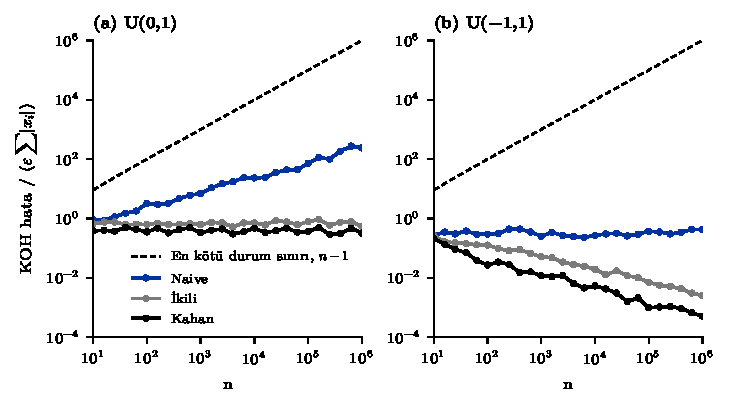
\includegraphics[width=0.86\linewidth]{../figures/tr/fig1_error_growth.pdf}
\caption{Üç yöntemin 30 dizi üzerinden KOH hatası, $\varepsilon\sum|x_i|$ biriminde. Kesikli çizgi: naive toplamanın en kötü
durum sınırı.}\label{fig:buyume}
\end{figure}

\textbf{Bulgu.} Pozitif terimlerde, $\mathrm{U}(0,1)$, naive hata bu ölçekte \SlopeNaivePos{} eğimle büyür: yuvarlama
hataları birbirinden bağımsız rastgele işaretli gibi davrandığında öngörüldüğü gibi $\sqrt{n}$ hızında (Johnson, 2019).
$n = 10^6$'da hata \NormNaivePos{} birimdir; sınır ise $10^6$'dır. İki işaretli terimlerde, $\mathrm{U}(-1,1)$, eğim yalnızca
\SlopeNaiveSym{}'dır: ara toplamlar küçük kaldığı için her yuvarlama hatası da küçüktür ve hata bir birimin altında kalır
($n = 10^6$'da \NormNaiveSym{}). Her iki durumda da ikili ve Kahan toplaması her $n$ için bir birimin altındadır ($n=10^6$'da
$\mathrm{U}(0,1)$ için \NormPairPos{} ve \NormKahanPos{}; $\mathrm{U}(-1,1)$ için \NormPairSym{} ve \NormKahanSym{}).

\textbf{Yorum.} ``Hata doğrusal büyür'' ifadesi tipik davranışı değil, sınırı anlatır. Hatanın gerçekte ne hızla büyüdüğü,
ara toplamların büyüklüğü aracılığıyla veriye bağlıdır.

\section{Analiz 2: Koşul sayısı (Şekil~\ref{fig:kosul})}

\textbf{Neden.} 1.\ sürümde göreli hata çalıştırmadan çalıştırmaya çok değişiyordu. Naive sınır $|S|$'ye bölününce
$|E|/|S| \le \gamma_{n-1}\,\kappa$ elde edilir; $\kappa = \sum|x_i|/|\sum x_i|$ toplamın koşul sayısıdır. İki işaretli
terimler birbirini neredeyse götürdüğünde $|S|$ küçük, $\kappa$ büyük olur; böylece küçük bir mutlak hata bile büyük bir göreli
hataya dönüşür. Bu analiz, değişkenliği $\kappa$'nın açıklayıp açıklamadığını sınar.

\textbf{Yöntem.} $\mathrm{U}(-1,1)$'den $n = 10^4$ elemanlı \CondTrials{} dizi; her biri için $\kappa$ ile naive ve Kahan
toplamının kesin göreli hatası.

\textbf{Şekil nasıl okunur?} Her nokta bir dizidir. Noktaların sağa doğru yükselmesi, göreli hatanın koşul sayısını izlediği
anlamına gelir.

\begin{figure}[h]
\centering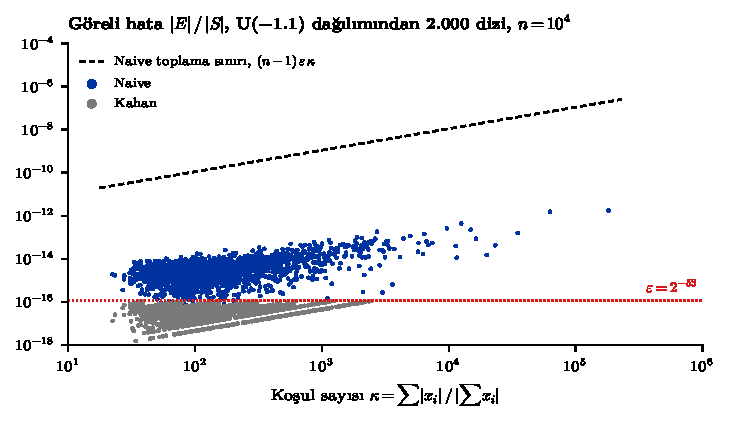
\includegraphics[width=0.86\linewidth]{../figures/tr/fig2_conditioning.pdf}
\caption{$\mathrm{U}(-1,1)$'den $10^4$ elemanlı \CondTrials{} dizi için göreli hata ve koşul sayısı. Kesikli çizgi: naive
toplama sınırı. Noktalı çizgi: $\varepsilon$.}\label{fig:kosul}
\end{figure}

\textbf{Bulgu.} $\kappa$'nın medyanı \KappaMedian{}, en büyük değeri \KappaMax{}'dir. Naive göreli hata $\kappa$ ile
yükselir (log--log ölçekte eğim \CondSlope{}) ve sınırın çok altında kalır (\BoundViolations{} ihlal). Ortalaması,
$\RelMean$, medyanının ($\RelMedian$) \MeanOverMedian{} katıdır; çünkü en büyük hatalı \%1'lik dilim ortalamanın
\%\TopShare'sini oluşturur: 1.\ sürümdeki gibi göreli hataların ortalaması, sıfıra yakın birkaç toplamın etkisi altındadır.
Kahan'ın göreli hatası $\kappa$ ne olursa olsun \KahanMaxEps{}$\,\varepsilon$'u aşmaz; noktalarının bantlar oluşturmasının
nedeni, sonucun kesin toplamdan en fazla bir yuvarlama uzakta olması ve yuvarlamanın kesikli adımlarla gerçekleşmesidir.

\textbf{Yorum.} ``Dalgalanma'' yöntemin kararsızlığı değil, problemin koşulluluğudur. Naive toplama geriye doğru
kararlıdır: $\hat S$, girdilerin en fazla $\gamma_{n-1}$ oranında bozulmuş hâllerinin kesin toplamıdır (Higham, 2002,
4.\ bölüm; Johnson, 2019). Kötü koşullu bir toplamda büyük göreli hata, geriye doğru kararlı her yöntemin üretebileceği bir
sonuçtur.

\section{Analiz 3: Yöntemler ve 1.\ sürümün referansı (Tablo~\ref{tab:yontem})}

\textbf{Neden.} Daha doğru bir yöntem, ancak maliyeti kabul edilebilirse kullanılmaya değer; bu yüzden doğruluk ve süre birlikte
ölçüldü. 1.\ sürüm kesin toplam olarak {\XeTeXinterchartokenstate=0 \texttt{np.sum(x, dtype=np.longdouble)}} kullanmıştı; \texttt{longdouble}'ın duyarlılığı
platformdan platforma değişir (NumPy belgeleri). Bu nedenle onun doğruluğu da ölçüldü.

\textbf{Yöntem.} 1.\ sürümdeki gibi $\mathrm{U}(-1,1)$'den $10^6$ elemanlı 10 dizi. Hatalar 1.\ analizdeki gibi; süre beş
çağrının medyanıdır (\Machine).

\begin{table}[h]
\centering\footnotesize
\caption{$n = 10^6$ için $\varepsilon\sum|x_i|$ biriminde KOH hata ve çalışma süresi.}\label{tab:yontem}
\begin{tabular}{lrr}
\toprule
Yöntem & KOH hata & Süre (ms) \\
\midrule
Naive, Python döngüsü (sürüm 1) & 0{,}442 & 17{,}86 \\
Naive, \texttt{np.cumsum} & 0{,}442 & 2{,}09 \\
İkili & $1{,}9\times 10^{-3}$ & 0{,}47 \\
\texttt{np.sum} (NumPy, kısmi ikili) & $2{,}4\times 10^{-3}$ & 0{,}13 \\
Kahan, Python döngüsü & $4{,}2\times 10^{-4}$ & 67{,}10 \\
\texttt{math.fsum} (doğru yuvarlanmış) & $4{,}2\times 10^{-4}$ & 15{,}13 \\
\texttt{np.sum}, \texttt{longdouble} (sürüm 1 referansı) & $2{,}4\times 10^{-3}$ & 0{,}13 \\
\bottomrule

\end{tabular}
\end{table}

\textbf{Bulgu.} 1.\ sürümün Python döngüsü hem isabetsiz hem yavaştır: \TimeLoop{} ms sürer. Sonucu kesin toplamın doğru
yuvarlanmış hâli olan \texttt{math.fsum} ise \TimeFsum{} ms sürer (\LoopOverFsum{} kat hızlı); \texttt{np.sum} de \TimeNpSum{}
ms'de, iki basamak daha küçük bir hatayla sonuç verir. Kahan yöntemi \texttt{fsum}'un doğruluğuna ulaşır ama Python'da
yazıldığında yavaştır (\TimeKahan{} ms); avantajı, terim başına yalnızca sabit miktarda ek iş gerektirmesidir ve bu, derlenmiş
kodda önemlidir. \LongdoubleSentence. Burada yapıldığı gibi hataları kesin bir referansla ölçmek bu platform bağımlılığını
ortadan kaldırır.

\section{Sonuç ve sınırlılıklar}

\begin{itemize}
  \item Naive toplamanın hatası en kötü durum sınırının çok altındadır. Aynı işaretli terimlerde sınırın ölçeğinde $\sqrt{n}$
  hızında büyür, birbirini götüren terimlerde ise neredeyse hiç büyümez. Göreli hatayı koşul sayısı belirler.
  \item Naive toplama kararsız değil, geriye doğru kararlıdır. Python'da doğru toplam için \texttt{math.fsum} hem doğru
  yuvarlanmış sonuç verir hem de Python döngüsünden hızlıdır; \texttt{np.sum} hızlıdır ve naive toplamadan çok daha doğrudur.
  \item Yalnızca tekdüze veri, çift duyarlılık ve $10^6$'ya kadar boyutlar incelendi. Süreler tek bir makinede ölçüldü.
\end{itemize}

\section*{Kaynaklar}
{\small
Higham, N. J. (1993). The accuracy of floating point summation. \textit{SIAM J.\ Scientific Computing}, 14(4), 783--799.\\
Higham, N. J. (2002). \textit{Accuracy and Stability of Numerical Algorithms}, 2.\ baskı. SIAM.\\
Johnson, S. G. (2019). Notes on the accuracy of naive summation; Backwards stability of recursive summation.
MIT 18.335J, \textit{Introduction to Numerical Methods}, 3.\ ders.\\
Kahan, W. (1965). Further remarks on reducing truncation errors. \textit{Communications of the ACM}, 8(1), 40.\\
NumPy belgeleri: \texttt{numpy.sum}, \texttt{numpy.cumsum}, \texttt{numpy.finfo}. Python belgeleri: \texttt{math.fsum}.

\smallskip
Kodun yazımında ve bu notun hazırlanmasında bir yapay zekâ kodlama asistanından yararlanılmıştır. Tüm sayılar
\texttt{figures/*.csv} dosyalarından \texttt{make\_paper.py} ile üretilir.
}

\end{document}
